% PREAMBLE
%
% author: Daniel Wehner

% list of use-packages
% ------------------------------------------------------------------------------------
\usepackage[utf8]{inputenc}	% utf-8 input encoding
% language package
\usepackage[georgian,russian,english]{babel}

% citation and bibliography
\usepackage{cite}				% citation
\usepackage[round]{natbib} 		% citation (<author>, <year>)
%\bibliographystyle{plainnat}

\usepackage{varioref}			% cross references
% hyper-references
\usepackage[hyphens]{url}
\usepackage[colorlinks=true,linkcolor=black,citecolor=blue]{hyperref}

% images and graphics
\usepackage{tikz}				% tikz image creation
\usepackage{picture}
\usepackage{pgfplots} 		% plots
\usepackage{graphicx} 		% display images

\usetikzlibrary{shapes}
\usetikzlibrary{patterns}
\usetikzlibrary{tikzmark}
\usetikzlibrary{decorations.pathreplacing}

% tables
\usepackage{array}
\usepackage{tabularx} 		% special type of table, allows to specify the width of columns
\usepackage{longtable} 		% table over several pages (also needed for acronyms)
\usepackage{makecell} 		% line-break in table cells
\usepackage{booktabs} 		% table lines, ...
\usepackage{multirow}		% extent cells over more table rows

% math
\usepackage{bm}				% bold face math
\usepackage{nicefrac}			% nice fractions
\usepackage{amsmath} 		% math scripts
\usepackage{mathtools} 		% math scripts and tools
\usepackage[mathscr]{eucal} 	% math scripts

% color
\usepackage{xcolor} 			% color package
\usepackage{colortbl} 		% colored tables (cellcolor, ...)
\usepackage[many]{tcolorbox}	% colored boxes

% misc
\usepackage{soul} 			% fonts
\usepackage{float}
\usepackage{pifont} 			% symbols
\usepackage{blkarray}		% blockarray
\usepackage{mxedruli} 		% Georgian script
\usepackage{fontawesome} 	% symbols
\usepackage[normalem]{ulem}	% dashed / dotted underline

\usepackage{lscape} 			% landscape orientation
\usepackage{wrapfig}			% wrap figure in text
\usepackage{adjustbox} 		% rotation of content
\usepackage{enumitem} 		% enumeration

\usepackage{etoolbox}

% glossary
\usepackage[acronym,nonumberlist,nopostdot,nogroupskip=true]{glossaries}
\makeglossaries

% just for testing
\usepackage{blindtext}


% settings + definitions
% ------------------------------------------------------------------------------------

% spacing
\setlength{\parskip}{\baselineskip} % spacing after paragraph
\setlength{\parindent}{0pt} 		% no indent

% glossary / acronym
\newglossarystyle{mylong}{%
  	\setglossarystyle{long}%
  	\renewcommand{\glossentry}[2]{%
    		\glsentryitem{##1}\glstarget{##1}{\bfseries \glossentryname{##1}} &
    		~~~~~~\glossentrydesc{##1}\glspostdescription\space ##2\tabularnewline
  	}%
}
\setglossarystyle{mylong}

\makeatletter
\pretocmd{\section}{\addtocontents{toc}{\protect\addvspace{16.5\p@}}}{}{}
\pretocmd{\subsection}{\addtocontents{toc}{\protect\addvspace{5\p@}}}{}{}
\pretocmd{\subsubsection}{\addtocontents{toc}{\protect\addvspace{5\p@}}}{}{}
\makeatother

\addto\captionsenglish{%
	\renewcommand{\contentsname}%
	{Table of Contents}%
}

% color definitions
% ------------------------------------------------------------------------------------
\definecolor{gold}{rgb}{0.99, 0.76, 0.0}
\definecolor{silver}{rgb}{0.75, 0.75, 0.75}
\definecolor{bronze}{rgb}{0.76, 0.23, 0.13}

% commands
% ------------------------------------------------------------------------------------

% TEXT ~~~~~~~~~~~~~~~~~~~~~~~~~~~~~
% highlight command
\newcommand{\highlight}[1]{\textcolor{tud9c}{\textbf{#1}}}

% linkstyle command
\newcommand{\linkstyle}[1]{\textcolor{blue}{\underline{\smash{\texttt{#1}}}}}

% subscript in text
\newcommand{\ssc}[1]{$_{\text{#1}}$}
\newcommand{\underl}[1]{\underline{\smash{#1}}}

% circled number
\newcommand{\circled}[1]{\tikz[baseline=(char.base)]{\node[shape=circle,draw,inner sep=1pt] (char) {\scriptsize #1};}}
\newcommand{\circledBlk}[1]{\tikz[baseline=(char.base)]{
	\node[shape=circle,draw,fill=black,inner sep=1pt,thick] (char) {\scriptsize \textcolor{white}{\textbf{#1}}};}
}

% cmark and xmark
\newcommand{\cmarkgr}{\textcolor{green!30!black}{\textbf{\ding{51}}}}
\newcommand{\bmarkor}{\textcolor{orange}{\textbf{\ding{93}}}}
\newcommand{\xmark}{\textcolor{red}{\textbf{\ding{55}}}}

% TABLES ~~~~~~~~~~~~~~~~~~~~~~~~~~~~
% cellcolors in table
\newcommand{\cgr}{\cellcolor{green!10}\cmarkgr}
\newcommand{\cor}{\cellcolor{orange!10}\bmarkor}
\newcommand{\cre}{\cellcolor{red!10}\xmark}
\newcommand{\cgb}{\cellcolor{black}}
\newcommand{\gry}[1]{\cellcolor{lightgray!60} #1}
\newcommand{\gr}{\cellcolor{lightgray}}

% thick vertical lines in tables (instead of | c | -> ? c ?)
\newcolumntype{?}{!{\vrule width 1.5pt}}

% centered X column
\newcolumntype{Y}{>{\centering\arraybackslash}X}

% rotated cell content
\newcolumntype{R}[2]{%
    >{\adjustbox{angle=#1,lap=\width-(#2)}\bgroup}%
    l%
    <{\egroup}%
}
\newcommand*\rot{\multicolumn{1}{R{90}{1em}}}
\newcommand*\rotff{\multicolumn{1}{R{45}{1em}}}

% BOXES ~~~~~~~~~~~~~~~~~~~~~~~~~~~~~
% box
\newtcolorbox{tudbox}[1]{colback=white,colframe=tud9c!70,fonttitle=\bfseries,title=\textcolor{white}{#1}}

% adjusted colorbox
\newcommand{\cbox}[2]{%
  	\begingroup\setlength{\fboxsep}{1pt}%
  	\colorbox{#1}{\texttt{\hspace*{4pt}\vphantom{Ay}#2\hspace*{4pt}}}%
  	\endgroup
}

% embedding pictures in table cells
\newcommand{\AddCellBackground}[4][\tabcolsep]{%
  	\unskip\begin{picture}(0,0)
    		\put(-#1,-\dp\strutbox){\includegraphics[width=\dimexpr
      		#2+\dimexpr #1*2\relax\relax,height=#3]{#4}}%
  	\end{picture}\ignorespaces
}

% MISC     ~~~~~~~~~~~~~~~~~~~~~~~~~~~~

\newcommand{\github}{\makebox[0.5cm][r]{\raisebox{-0.4ex}{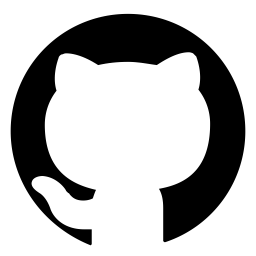
\includegraphics[scale=0.04]{images/github}}}}
